\section{Image Coordinates}
\subsection{Image Coordinate System}
Sensor Coordinates:
\begin{itemize}
    \item The pixel-based, discrete coordinate system used in digital images.
    \item Origin: Top-left corner of the image.
    \item coordinates increasing to the right (x+-axis) and downward (y+-axis)
    \item \(u \rightarrow x, v \rightarrow y\)
\end{itemize}
Metric Cartesian Coordinates:
\begin{itemize}
    \item Continuous coordinate system used in image processing.
    \item Origin: Center of the image.
\end{itemize}

Camera Coordinate Systems:
\begin{figure}[ht]
    \centering
    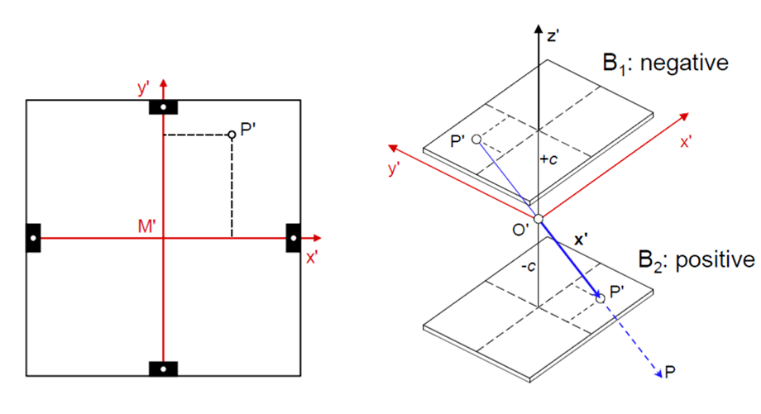
\includegraphics[width = \columnwidth]{Images/08/CameraCoordinateSystems.png}
    \caption{Camera Coordinate System}
    \label{fig:camera_coordinate_system}
\end{figure}
Paramters:
\begin{itemize}
    \item Image coordinate system origin (M', H', O')
    \item Camera constant c
\end{itemize}
are basic intrinsic camera parameters or
camera-intrinsics
\subsection{Transformation between Sensor and Cartesian Coordinates}
\[
x' = -\frac{s_x}{2} + \Delta x_s \cdot u
\]
\[
y' = \frac{s_y}{2} - \Delta y_s \cdot v
\]
Formulae implies the origin of the Cartesian coordinate system at the middle of the sensor \(\rightarrow\) That is rarely correct.

\subsection{Pinhole Camera: Approximation of an imperfect system!}
Physical camera is affected by a variety of error sources:
\begin{itemize}
    \item Lens distortion
    \item Non-planar sensor surface
    \item Temperature effects
\end{itemize}
Intrinsic parameters are computed through the camera calibration procedure.

\subsection{Homogeneous Coordinates}
\begin{itemize}
    \item \(K\): Camera matrix
    \item \(R\): Rotation matrix(orthonormal)
    \item \(t\): Translation vector
    \item \(\mathbf{x}\): Homogeneous image coordinates
    \item \(\mathbf{X}_{world}\): World coordinates
\end{itemize}
\[
\mathbf{x} = K \cdot [R | t] \cdot \mathbf{X}_{world}
\]


\[
\mathbf{x}_h =
\begin{bmatrix}
x_h \\
y_h \\
z_h \\
w
\end{bmatrix}
\qquad
\mathbf{x} =
\begin{bmatrix}
x_h / w \\
y_h / w \\
z_h / w \\
w / w
\end{bmatrix}
=
\begin{bmatrix}
x \\
y \\
z \\
1
\end{bmatrix}
\]

\[
\mathbf{X} =\mathbf{T}\cdot \mathbf{x}
\]
\[
\mathbf{T} =
\left[
\begin{array}{ccc|c}
a_{11} & a_{12} & a_{13} & a_{14} \\
a_{21} & a_{22} & a_{23} & a_{24} \\
a_{31} & a_{32} & a_{33} & a_{34} \\
\hline
a_{41} & a_{42} & a_{43} & a_{44}
\end{array}
\right]
=
\begin{bmatrix}
\mathbf{T}_{11} & \mathbf{T}_{12} \\
\mathbf{T}_{21} & \mathbf{T}_{22}
\end{bmatrix}
\]
\[
\begin{array}{rl}
\mathbf{T}_{11} : & \text{scaling, reflection in a line, rotation} \\
\mathbf{T}_{12} : & \text{translation} \\
\mathbf{T}_{21} : & \text{perspective} \\
\mathbf{T}_{22} : & \text{homogeneous scaling (factor } w\text{)}
\end{array}
\]
For exact matrices (for scale, rotation) see Presentation slides.
\subsection{Basic coordinate systems and the operations on them}
\textbf{Rigid registration = Similarity transformation}
\[
\mathbf{X} = \mathbf{A} \cdot \mathbf{x} + \mathbf{a}
\]
\[
\mathbf{X} = m \cdot \mathbf{R} \cdot \mathbf{x} + \mathbf{X}_0
\]
with 
\[
\mathbf{R} =
\begin{bmatrix}
\cos(\alpha) & -\sin(\alpha) \\
\sin(\alpha) & \cos(\alpha) \\
\end{bmatrix}
\]
\textbf{Polynomial Transformation}
\[
X = \sum_{j=0}^{n} \sum_{i=0}^{j} a_{ji} \cdot x^{j-i} \cdot y^{i}
\]

\[
Y = \sum_{j=0}^{n} \sum_{i=0}^{j} b_{ji} \cdot x^{j-i} \cdot y^{i}
\]

\subsubsection{Projective Transformation}
3D Space to Plane Mapping

\textbf{Central Projection:}

\[
X = \frac{a_0 + a_1 \cdot x + a_2 \cdot y}{1 + c_1 \cdot x + c_2 \cdot y}
\]

\[
Y = \frac{b_0 + b_1 \cdot x + b_2 \cdot y}{1 + c_1 \cdot x + c_2 \cdot y}
\]

\[
a_0 + a_1 x + a_2 y - X - c_1 x X - c_2 y X = 0
\]

\[
b_0 + b_1 x + b_2 y - Y - c_1 x Y - c_2 y Y = 0
\]
\textbf{Homography:} Plane to Plane transformation
\[
\begin{bmatrix}
x_2 \\
y_2 \\
z_2
\end{bmatrix}
=
\begin{bmatrix}
H_{11} & H_{12} & H_{13} \\
H_{21} & H_{22} & H_{23} \\
H_{31} & H_{32} & H_{33}
\end{bmatrix}
\begin{bmatrix}
x_1 \\
y_1 \\
z_1
\end{bmatrix}
\quad \Leftrightarrow \quad
\mathbf{x}_2 = H \mathbf{x}_1
\]
with \(x'_2 = x_2/z_2\) and \(y'_2 = y_2/z_2\)

\[
x'_2 = \frac{H_{11}x_1 + H_{12}y_1 + H_{13}z_1}{H_{31}x_1 + H_{32}y_1 + H_{33}z_1}
\]

\[
y'_2 = \frac{H_{21}x_1 + H_{22}y_1 + H_{23}z_1}{H_{31}x_1 + H_{32}y_1 + H_{33}z_1}
\]
Create 4 equation pairs to solve projection problem using eigenvalue decomposition…
\subsection{Overview Transformations}
Isometric Transformation:
\[
\mathbf{x}' = 
\begin{pmatrix}
R & \mathbf{t} \\
\mathbf{0}^\mathrm{T} & 1
\end{pmatrix}
\mathbf{x}
\]

Similarity Transformation:
\[
\mathbf{x}' = 
\begin{pmatrix}
sR & \mathbf{t} \\
\mathbf{0}^\mathrm{T} & 1
\end{pmatrix}
\mathbf{x}
\]
Affine Transformation:
\[
\mathbf{x}' = 
\begin{pmatrix}
A & \mathbf{t} \\
\mathbf{0}^\mathrm{T} & 1
\end{pmatrix}
\mathbf{x}
\]

\[
A = R(\theta) R(-\phi) D R(\phi)
\]

\[
D = 
\begin{pmatrix}
\lambda_1 & 0 \\
0 & \lambda_2
\end{pmatrix}
\]
Homography:

\[
\mathbf{x}' = 
\begin{pmatrix}
A & \mathbf{t} \\
\mathbf{v}^\mathrm{T} & v
\end{pmatrix}
\mathbf{x}
\]

\subsection{Distortions}
All effects are caused by different aperture
positions.
\begin{itemize}
    \item Barrel distortion effect
    \item Cushion distortion effect
    \item Chromatic abberation (Color Error)
\end{itemize}